\documentclass{article}%
\usepackage[T1]{fontenc}%
\usepackage[utf8]{inputenc}%
\usepackage{lmodern}%
\usepackage{textcomp}%
\usepackage{lastpage}%
\usepackage[head=40pt,margin=0.5in,bottom=0.6in]{geometry}%
\usepackage{graphicx}%
%
\title{\textbf{Encovi: Cantidad de hogares pobres en Venezuela aumentó 48\% en 2018}}%
\author{EL NACIONAL WEB}%
\date{30/11/2018}%
%
\begin{document}%
\normalsize%
\maketitle%
\textbf{URL: }%
http://www.el{-}nacional.com/noticias/sociedad/encovi{-}cantidad{-}hogares{-}pobres{-}venezuela{-}aumento{-}2018\_261657\newline%
%
\textbf{Periodico: }%
EN, %
ID: %
261657, %
Seccion: %
Sociedad\newline%
%
\textbf{Palabras Claves: }%
Sociedad\newline%
%
\textbf{Derecho: }%
2.10, %
Otros Derechos: %
, %
Sub Derechos: %
2.10.1\newline%
%
\textbf{EP: }%
NO\newline%
\newline%
%
\textbf{\textit{La directora del Instituto de Investigaciones Económicas y Sociales de la Universidad Católica Andrés Bello informó que la escasez de alimentos y de servicios de públicos impide que los niños asistan a las aulas de clase}}%
\newline%
\newline%
%
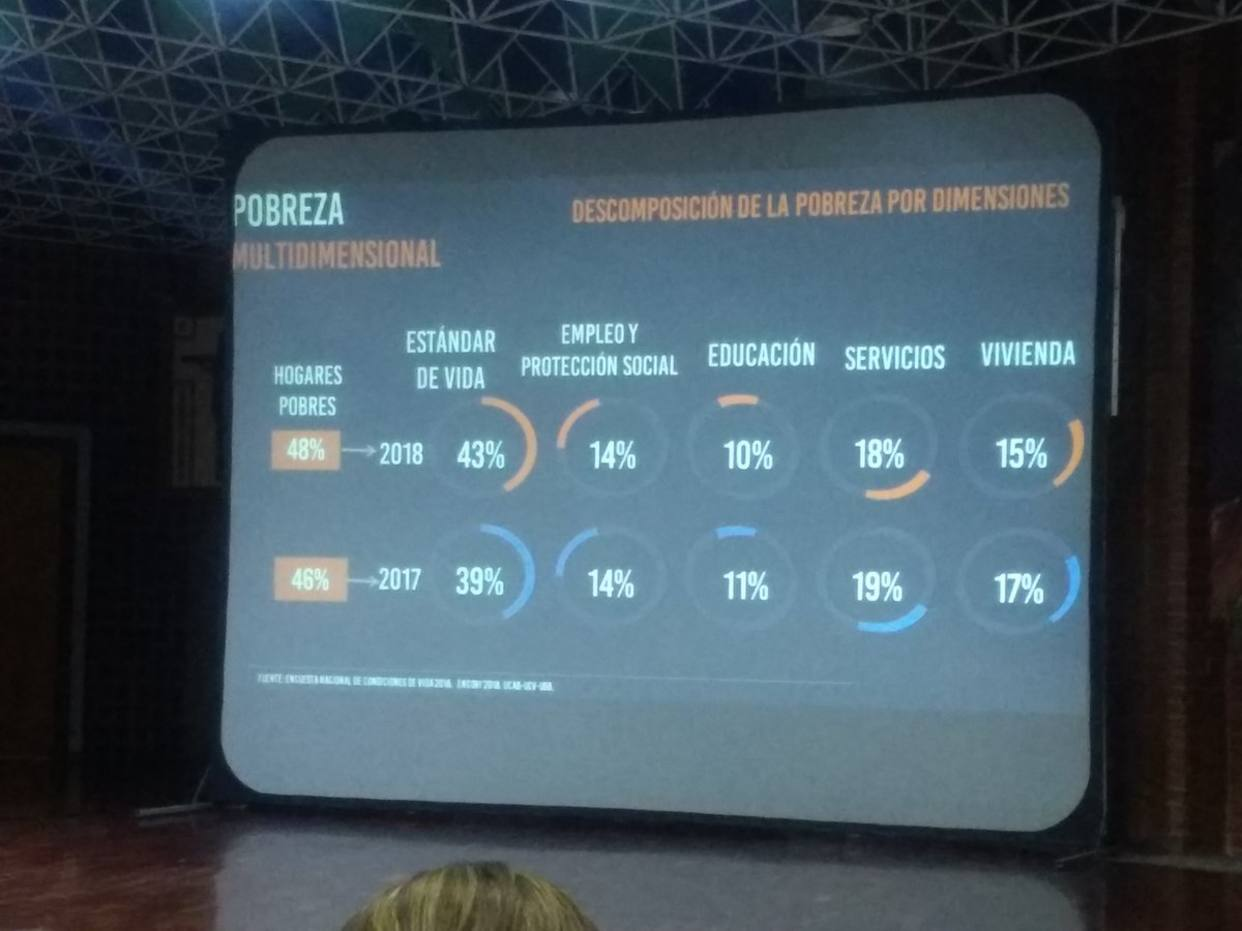
\includegraphics[width=300px]{40.jpg}%
\newline%
%
Anitza Freitez, directora del Instituto de Investigaciones Económicas y Sociales de la Universidad Católica Andrés Bello, compartió los resultados preliminares de la Encuesta Nacional de Condiciones de Vida (Encovi).%
\newline%
%
Freitez informó este viernes que, de acuerdo con el estudio,~~la cantidad de~hogares pobres de Venezuela incrementó a 48\% durante el año 2018.%
\newline%
%
Además, los resultados preliminares de la encuesta arrojaron que la falta de agua, transporte y comida representan las principales razones por la que los niños no asisten a clases.%
\newline%
%
El estudio señala~que la migración educativa de colegio privados a públicos aumentó debido a que~los padres de los estudiantes~no pueden pagar las mensualidades.%
\newline%
%
"Más del 76\% de la población, comprendida entre los 18 y 24 años, ha migrado a las instituciones y planteles públicos durante el 2018.%
\newline%
%
\end{document}